\documentclass[11pt]{article}

\usepackage[margin=1in]{geometry}
\usepackage{amsmath}
\usepackage{amssymb}
\usepackage{amsthm}
\usepackage{booktabs}
\usepackage{enumitem}
\usepackage{graphicx}
\usepackage{hyperref}
\usepackage{tikz}
\usetikzlibrary{arrows.meta, positioning, shapes.geometric}

\hypersetup{
  colorlinks=true,
  linkcolor=blue,
  urlcolor=blue,
  citecolor=blue
}

\newtheorem{assumption}{Assumption}
\newtheorem{proposition}{Proposition}
\newtheorem{definition}{Definition}
\newtheorem{remark}{Remark}

\newcommand{\simplex}{\Delta^{N-1}}
\newcommand{\E}{\mathbb{E}}
\newcommand{\R}{\mathbb{R}}
\newcommand{\Var}{\mathrm{Var}}
\newcommand{\KL}{\mathrm{KL}}
\newcommand{\1}{\mathbf{1}}
\newcommand{\code}[1]{\texttt{\detokenize{#1}}}
\newcommand{\pathref}[1]{\texttt{\detokenize{#1}}}

\title{Regime-Aware Proximal Policy Optimization for Long-Only Portfolio Control}
\author{Anonymous Authors}
\date{}

\begin{document}

\maketitle

\begin{abstract}
We study a regime-aware reinforcement learning formulation for long-only
portfolio allocation under transaction costs, drawdown penalties, and
walk-forward evaluation. The proposed framework couples three ideas that are
often treated separately in quantitative trading systems: causal market-state
representation learning, filtering-only latent regime inference, and constrained
policy optimization on the probability simplex. Market histories are embedded
into a low-dimensional state by temporal and cross-sectional encoders; latent
regime probabilities are obtained from a Gaussian hidden Markov model using
forward filtering only; and a Proximal Policy Optimization (PPO) actor-critic
agent parameterizes portfolio weights with a Dirichlet policy. We formalize the
resulting decision process, derive the implemented clipped surrogate objective,
and characterize the role of transaction-cost and drawdown terms in the reward.
The paper also describes an auditable reference implementation in JAX, designed
for deterministic walk-forward evaluation on public market data. Our analysis
highlights the practical gap between a minimal mathematically transparent PPO
portfolio optimizer and a more stable trainer, showing how optimizer state,
minibatching, KL diagnostics, value-target freezing, and critic clipping are
incorporated without changing the causal walk-forward protocol.
\end{abstract}

\section{Introduction}

Portfolio construction is naturally sequential: each rebalance changes not only
current exposure but also future cash drag, transaction costs, drawdown, and
risk capacity. Reinforcement learning (RL) is therefore an attractive modeling
language for portfolio control. However, financial RL systems are unusually easy
to overstate. Non-causal preprocessing, smoothed regime labels, poorly specified
cash accounting, and optimistic backtests can dominate any apparent algorithmic
gain.

This paper formulates and analyzes a regime-aware PPO framework for long-only
portfolio control. The method is motivated by a simple premise: before pursuing
complex agents, the full research stack should be vertically functional,
deterministic, and auditable. The reference implementation follows this premise:
public market data are converted into split-safe features, market states are
encoded from causal lookback windows, latent regimes are inferred by filtering,
and PPO is trained on frozen train windows before evaluation on future test
windows.

The main contributions are:
\begin{enumerate}[leftmargin=*]
  \item A formal Markov decision process for long-only portfolio allocation with
  transaction costs, drawdown penalties, benchmark-relative rewards, and
  portfolio-context state.
  \item A regime-aware state construction that combines learned market embeddings
  with filtering-only HMM posterior probabilities, avoiding forward-backward
  smoothing and future regime information.
  \item A simplex-valued PPO actor based on a Dirichlet policy, enabling direct
  stochastic exploration over target portfolio weights.
  \item A conference-style theoretical and algorithmic description of a compact
  JAX reference implementation, including its exact loss, stabilized PPO update
  loop, tensor shapes, diagnostics, and limitations.
\end{enumerate}

\section{Problem Formulation}

Let $(\Omega,\mathcal{F},\{\mathcal{F}_t\}_{t\ge0},\Pr)$ be a filtered
probability space representing market information through rebalance time $t$.
All quantities used to form a decision at time $t$ must be
$\mathcal{F}_t$-measurable. This measurability condition is the mathematical
version of the implementation rule that no preprocessing, regime inference, or
policy input may depend on future rows. Let there be $N$ tradable assets,
including cash when cash is available as an explicit return series. At each
rebalance time $t$, the agent selects target weights
\[
a_t = w^{\mathrm{target}}_t \in \simplex,
\qquad
\simplex = \{w \in \R^N : w_i \ge 0,\ \sum_i w_i = 1\}.
\]
The environment executes long-only normalized weights $\hat{w}_t$, observes
holding-period returns $R_t \in \R^N$, and updates wealth.

The decision chronology is:
\begin{enumerate}[leftmargin=*]
  \item At the decision date, the agent observes a causal state $s_t$ assembled
  from past and current features, filtering regime probabilities, and portfolio
  context.
  \item The policy samples a target allocation $a_t$ on the simplex.
  \item The environment normalizes the target allocation if needed, charges
  transaction cost for moving from $w_{t-1}$ to $\hat{w}_t$, and then applies
  the holding-period return $R_t$.
  \item The next portfolio context $(w_t,d_t,\tau_t)$ is carried into the next
  decision.
\end{enumerate}
This ordering matters. Transaction cost depends on the rebalance decision, but
the asset return is not known until after the decision. Therefore the action is
causal even though the reward is computed from the subsequent holding-period
return.

\begin{definition}[Portfolio State]
The state used by the policy is
\[
s_t =
\begin{bmatrix}
\phi_t \\
p_t \\
w_{t-1} \\
d_{t-1} \\
\tau_{t-1}
\end{bmatrix}
\in \R^{D_\phi + K + N + 2},
\]
where $\phi_t$ is a market embedding, $p_t \in \Delta^{K-1}$ is the filtering
posterior over latent regimes, $w_{t-1}$ is the current portfolio, $d_{t-1}$ is
current drawdown, and $\tau_{t-1}$ is previous turnover.
\end{definition}

This state intentionally contains portfolio context. Two histories with the same
market observation may require different actions if one portfolio is already
concentrated, has incurred recent turnover, or is in drawdown.

\begin{remark}[Why portfolio context is part of the Markov state]
The trading environment updates wealth and drawdown recursively. If the policy
were given only $\phi_t$ and $p_t$, it would not know the current weights and
therefore could not reason about turnover cost. It also would not know whether
the portfolio is near a drawdown penalty region. Including
$(w_{t-1},d_{t-1},\tau_{t-1})$ makes the state sufficient for the implemented
one-step accounting transition: given $s_t$, action $a_t$, and return $R_t$,
the environment can compute the next context without hidden mutable state.
\end{remark}

For a train/test split, let $\mathcal{T}_{\mathrm{train}}$ and
$\mathcal{T}_{\mathrm{test}}$ denote ordered rebalance indices with
\[
\max \mathcal{T}_{\mathrm{train}} < \min \mathcal{T}_{\mathrm{test}}.
\]
All fitted objects used by the policy checkpoint---preprocessors, HMM
parameters, actor parameters, critic parameters, and optimizer state---are
functions only of train data. The test period is then an out-of-sample
evaluation of a frozen checkpoint. This is not merely an experimental
convention: it is the condition that lets empirical returns be interpreted as a
causal backtest rather than an in-sample optimization trace.

\section{Causal Market Representation}

The market representation is produced from lookback windows ending at the
decision date. For lookback length $L$, asset count $A$, asset feature dimension
$F_a$, and macro feature dimension $F_m$, the encoder receives
\[
X^{asset}_t \in \R^{L \times A \times F_a},
\qquad
X^{macro}_t \in \R^{L \times F_m},
\qquad
X^{spectral}_t \in \R^{20}.
\]
A valid window at time $t$ has the form
\[
X^{asset}_t =
\left(x^{asset}_{t-L+1},x^{asset}_{t-L+2},\ldots,x^{asset}_{t}\right),
\]
and similarly for macro variables. Thus $X_t$ is
$\mathcal{F}_t$-measurable by construction. This is the first anti-leakage
barrier: any transformation that fits statistics using future rows would break
the measurability of $X_t$ and therefore invalidate the policy state.

A shared asset LSTM maps each asset's temporal window to a hidden vector, a
cross-asset attention layer models interactions among assets, attention pooling
produces a single market-wide asset embedding, and a macro LSTM embeds macro
history. The fused vector is mapped to
\[
\phi_t \in \R^{32}.
\]
Mathematically, the encoder is a deterministic map
\[
g_\eta:
\R^{L\times A\times F_a}\times \R^{L\times F_m}\times \R^{20}
\rightarrow \R^{32},
\qquad
\phi_t=g_\eta(X^{asset}_t,X^{macro}_t,X^{spectral}_t).
\]
If the encoder parameters $\eta$ are fixed before evaluating a split, then
$\phi_t$ inherits causality from the input windows. This is why the
implementation separates window construction, fitting, and evaluation: a
non-causal encoder can contaminate every later component, including HMM
posteriors and PPO actions.

\begin{figure}[ht]
\centering
\resizebox{\textwidth}{!}{
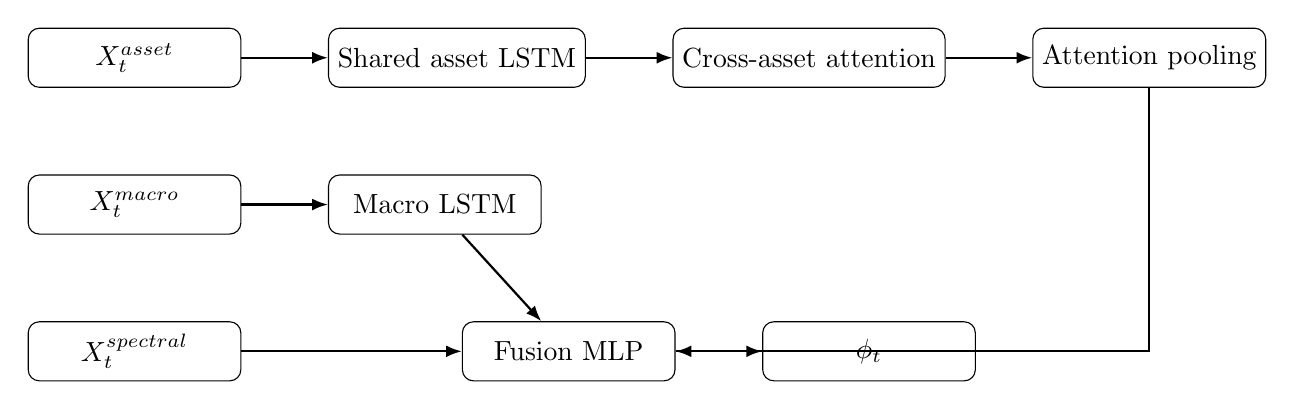
\begin{tikzpicture}[
  node distance=1.1cm,
  box/.style={draw, rounded corners, align=center, minimum width=2.7cm, minimum height=0.75cm},
  arrow/.style={-{Latex[length=2mm]}, thick}
]
\node[box] (asset) {$X^{asset}_t$};
\node[box, right=of asset] (alstm) {Shared asset LSTM};
\node[box, right=of alstm] (attn) {Cross-asset attention};
\node[box, right=of attn] (pool) {Attention pooling};
\node[box, below=of asset] (macro) {$X^{macro}_t$};
\node[box, right=of macro] (mlstm) {Macro LSTM};
\node[box, below=of macro] (spec) {$X^{spectral}_t$};
\node[box, right=2.8cm of spec] (fuse) {Fusion MLP};
\node[box, right=of fuse] (phi) {$\phi_t$};
\draw[arrow] (asset) -- (alstm);
\draw[arrow] (alstm) -- (attn);
\draw[arrow] (attn) -- (pool);
\draw[arrow] (macro) -- (mlstm);
\draw[arrow] (pool) |- (fuse);
\draw[arrow] (mlstm) -- (fuse);
\draw[arrow] (spec) -- (fuse);
\draw[arrow] (fuse) -- (phi);
\end{tikzpicture}
}
\caption{Causal market representation. Each decision uses only the current and
past observations contained in its lookback window.}
\end{figure}

\section{Filtering-Only Regime Inference}

Let $z_t \in \{1,\ldots,K\}$ denote an unobserved market regime. A diagonal
Gaussian HMM is fit on train embeddings $\phi_{1:T_{\mathrm{train}}}$ only.
Given fitted initial probabilities $\pi$, transition matrix $A$, means
$\mu_k$, and diagonal covariance matrices $\Sigma_k$, filtering computes
\[
p_t(k) = \Pr(z_t=k \mid \phi_{1:t})
\]
by the normalized forward recursion
\[
\alpha_t(k) \propto
\mathcal{N}(\phi_t;\mu_k,\Sigma_k)
\sum_j A_{jk}\alpha_{t-1}(j).
\]
More explicitly, write the emission density as
\[
b_k(\phi_t)=\mathcal{N}(\phi_t;\mu_k,\Sigma_k).
\]
The prediction and update steps are
\begin{align}
\tilde{\alpha}_t(k) &= \sum_{j=1}^{K}\alpha_{t-1}(j)A_{jk},\\
\bar{\alpha}_t(k) &= b_k(\phi_t)\tilde{\alpha}_t(k),\\
\alpha_t(k) &= \frac{\bar{\alpha}_t(k)}
{\sum_{\ell=1}^{K}\bar{\alpha}_t(\ell)}.
\end{align}
The output regime posterior is $p_t=\alpha_t$. This recursion has the same
shape as Bayesian filtering: first predict the next latent state using the
transition matrix, then update beliefs using the new observation. Each step is
causal because it uses only $\alpha_{t-1}$ and $\phi_t$.

No backward messages are used. This distinction is essential in finance:
forward-backward smoothing estimates $\Pr(z_t \mid \phi_{1:T})$ and therefore
uses future observations, which would leak information into the policy state.

\begin{remark}[Why filtering is enough for control]
For offline labeling tasks, smoothed regimes can be useful because the goal is
retrospective interpretation. For trading control, the policy must choose
$a_t$ before observing $\phi_{t+1:T}$. The filtering posterior
$\Pr(z_t\mid \phi_{1:t})$ is the correct belief state available to the agent.
Using $\Pr(z_t\mid \phi_{1:T})$ would train or evaluate the policy with
information that no deployed strategy could possess.
\end{remark}

\section{Portfolio Dynamics and Reward}

The environment maps target actions to executed long-only weights by projection
onto the simplex, denoted $\Pi_\Delta$:
\[
\hat{w}_t = \Pi_\Delta(a_t).
\]
For the Dirichlet actor, $a_t$ is already in $\simplex$ up to floating-point
roundoff, so $\Pi_\Delta$ is normally the identity. The projection remains in
the environment as a defensive accounting invariant: even if a future policy or
test fixture provides invalid weights, the executed portfolio remains
long-only and normalized.

Turnover, transaction cost, and return are
\begin{align}
\tau_t &= \sum_{i=1}^{N} |\hat{w}_{t,i} - w_{t-1,i}|,\\
c_t &= \rho \tau_t,\\
r^{gross}_t &= \hat{w}_t^\top R_t,\\
r^{net}_t &= r^{gross}_t - c_t.
\end{align}
The implemented turnover convention is the full $\ell_1$ distance between old
and new weights. If one instead reports one-way turnover, the value is
$\tau_t/2$. The full-distance convention is convenient for tests because the
maximum possible rebalance distance between two portfolios on the simplex is
exactly $2$.

Portfolio value and drawdown evolve as
\begin{align}
V_t &= V_{t-1}(1+r^{net}_t),\\
P_t &= \max(P_{t-1},V_t),\\
d_t &= 1 - V_t/P_t.
\end{align}
Here $P_t$ is the running peak value. Drawdown is path-dependent, which is why
the environment state carries both $V_t$ and $P_t$ internally and exposes
$d_t$ to the policy. If $V_t=P_t$, then $d_t=0$; if wealth falls below the
peak, $d_t$ is the fractional loss relative to that peak.

The scalar reward is benchmark-relative:
\[
\mathcal{R}_t =
\log(1+r^{net}_t)-\log(1+r^{b}_t)
- \lambda_d(d_t-d_{\max})_+
- \lambda_\tau \tau_t.
\]
The first two terms reward log excess return against the benchmark; the last
terms penalize drawdown-limit violations and turnover.

This reward can be read term by term. The log-return difference is
\[
\log(1+r^{net}_t)-\log(1+r^b_t)
=\log\left(\frac{1+r^{net}_t}{1+r^b_t}\right),
\]
so summing over time gives the log of cumulative relative wealth, ignoring
penalties:
\[
\sum_{t=1}^{T}
\left[\log(1+r^{net}_t)-\log(1+r^b_t)\right]
=
\log\left(
\frac{\prod_{t=1}^{T}(1+r^{net}_t)}
{\prod_{t=1}^{T}(1+r^b_t)}
\right).
\]
This additive property is the reason log excess return is convenient for PPO:
trajectory returns decompose into one-step rewards while still corresponding to
relative compounded performance. The drawdown term
$(d_t-d_{\max})_+$ is inactive until the drawdown exceeds the configured
tolerance, and the turnover term discourages policies that earn apparent alpha
only by excessive rebalancing.

\begin{remark}[Reward safety and domain]
The logarithms require $1+r^{net}_t>0$ and $1+r^b_t>0$. This is a natural
domain condition for weekly portfolio returns under ordinary long-only
backtests. If a future experiment permits leveraged losses below $-100\%$, the
reward definition would need an explicit clipping or default convention.
\end{remark}

\section{Dirichlet PPO on the Simplex}

\subsection{Policy Parameterization}

The actor network $f_\theta$ maps $s_t$ to logits $z_t \in \R^N$. The logits
define a mean allocation through temperature-scaled softmax:
\[
\mu_\theta(s_t) =
\operatorname{softmax}(z_t/T).
\]
Componentwise,
\[
\mu_{\theta,i}(s_t)
=
\frac{\exp(z_{t,i}/T)}
{\sum_{j=1}^{N}\exp(z_{t,j}/T)}.
\]
The temperature $T>0$ controls how sharply logits are converted into the mean
portfolio. Lower temperature makes the mean more concentrated; higher
temperature makes it closer to uniform, all else equal.

The stochastic policy is Dirichlet:
\[
\alpha_\theta(s_t) = c\,\mu_\theta(s_t)+\alpha_{\min}\mathbf{1},
\qquad
a_t \sim \pi_\theta(\cdot \mid s_t)
= \operatorname{Dirichlet}(\alpha_\theta(s_t)).
\]
This choice has two advantages. First, every sampled action lies on the
long-only simplex. Second, the concentration parameter $c$ separates the
network's mean allocation from exploration variance.

The mean of a Dirichlet random variable is
\[
\E[a_{t,i}\mid s_t]
=
\frac{\alpha_{\theta,i}(s_t)}
{\alpha_{\theta,0}(s_t)},
\qquad
\alpha_{\theta,0}(s_t)=\sum_{j=1}^{N}\alpha_{\theta,j}(s_t).
\]
Since $\alpha_\theta=c\mu_\theta+\alpha_{\min}\1$, this mean is close to
$\mu_\theta$ when $c$ is large relative to $N\alpha_{\min}$. The variance is
\[
\Var(a_{t,i}\mid s_t)=
\frac{\alpha_i(\alpha_0-\alpha_i)}
{\alpha_0^2(\alpha_0+1)}.
\]
Thus increasing $c$ increases $\alpha_0$ and reduces exploration variance
without changing the neural network architecture. This is useful in portfolio
control because the action has a hard budget constraint: exploration should
move around the simplex rather than leave it.

\subsection{Log Probability and Entropy}

For $a_t \in \simplex$ and $\alpha_0=\sum_i\alpha_i$, the log density is
\[
\log \pi_\theta(a_t\mid s_t)
= \log\Gamma(\alpha_0)
- \sum_i \log\Gamma(\alpha_i)
+ \sum_i(\alpha_i-1)\log a_i.
\]
The implementation clips action components inside the logarithm by a small
positive numerical floor. This does not change the intended support of the
Dirichlet policy; it prevents floating-point underflow when an action component
is extremely close to zero.

The Dirichlet entropy term used by the objective is
\[
H(\alpha) =
\sum_i \log\Gamma(\alpha_i)-\log\Gamma(\alpha_0)
+(\alpha_0-N)\psi(\alpha_0)
-\sum_i(\alpha_i-1)\psi(\alpha_i),
\]
where $\psi$ is the digamma function.

Entropy enters the loss with a negative sign, so larger entropy lowers the
minimized objective when $c_H>0$. In early experiments this can encourage
broader exploration over allocations. In later, more exploitation-oriented
experiments, the coefficient can be reduced or set to zero while the Dirichlet
concentration controls residual sampling noise.

\section{Advantage Estimation and PPO Objective}

The critic $V_\psi(s_t)$ estimates expected discounted return. Given trajectory
rewards and terminal masks $m_t=1-\mathrm{done}_t$, generalized advantage
estimation computes
\begin{align}
\delta_t &= \mathcal{R}_t + \gamma m_t V_\psi(s_{t+1}) - V_\psi(s_t),\\
A_t &= \delta_t + \gamma\lambda m_t A_{t+1},\\
G_t &= A_t + V_\psi(s_t).
\end{align}
The temporal-difference residual $\delta_t$ asks whether the realized reward
plus bootstrapped next value exceeded the critic's prediction. GAE then forms
an exponentially weighted sum of these residuals. The parameter $\lambda$
interpolates between low-variance one-step TD estimates and higher-variance
long-horizon Monte Carlo estimates:
\[
\lambda=0 \Rightarrow A_t=\delta_t,
\qquad
\lambda=1 \Rightarrow A_t
\approx
\sum_{\ell\ge0}\gamma^\ell \mathcal{R}_{t+\ell}-V_\psi(s_t),
\]
with terminal masks cutting the recursion at episode boundaries.

Advantages are standardized once over the rollout:
\[
\hat{A}_t = \frac{A_t-\bar{A}}{\sigma_A+\epsilon_{\mathrm{num}}}.
\]
In the implementation this normalization is guarded against near-zero standard
deviation; if the rollout advantages are numerically constant, normalized
advantages are set to zero rather than amplified by division by a tiny number.

Let $\theta_{\mathrm{old}}$ denote rollout policy parameters. PPO forms the
importance ratio
\[
r_t(\theta)=
\exp\{\log\pi_\theta(a_t\mid s_t)
-\log\pi_{\theta_{\mathrm{old}}}(a_t\mid s_t)\}.
\]
This ratio is the likelihood-ratio correction that lets samples from the old
policy estimate the objective of a nearby new policy:
\[
\E_{a\sim\pi_{\theta_{\mathrm{old}}}}
\left[
r_t(\theta)\hat{A}_t
\right]
=
\E_{a\sim\pi_{\theta}}
\left[
\hat{A}_t
\right],
\]
provided the two policies have compatible support. The Dirichlet floor
$\alpha_{\min}>0$ helps maintain that support on the simplex interior.

The clipped surrogate minimized in the implementation is
\[
L_\pi(\theta)
=-\frac{1}{T}\sum_{t=1}^{T}
\min\left(
r_t(\theta)\hat{A}_t,\,
\operatorname{clip}(r_t(\theta),1-\varepsilon,1+\varepsilon)\hat{A}_t
\right).
\]
The minimum is the core PPO safeguard. If an action with positive advantage
becomes much more likely than it was under the rollout policy, the clipped term
limits the gain. If an action with negative advantage becomes much less likely,
the clipped term similarly limits the improvement. In both cases, clipping
discourages policy updates that move too far from the data-generating policy in
one optimization phase.

After a rollout is collected, the implementation freezes the state-action
trajectory, old log probabilities, old critic values, normalized advantages,
and value targets. These tensors are then reused across all PPO epochs and
minibatches for that rollout.

Freezing is mathematically important. The old log probability in
$r_t(\theta)$ must describe the policy that actually generated $a_t$. If it
were recomputed after every parameter update, the ratio would collapse toward
one and no longer measure policy change. Similarly, recomputing GAE with the
moving critic during PPO epochs would make the target change while the optimizer
is trying to fit it, mixing policy improvement with target drift. The
implemented update therefore treats
\[
\mathcal{B}=
\{s_t,a_t,\log\pi_{\theta_{\mathrm{old}}}(a_t\mid s_t),
\hat{A}_t,G_t,V_{\mathrm{old},t}\}_{t=1}^{T}
\]
as a fixed batch for the duration of the PPO update.

The value function can be trained with the standard squared loss,
\[
L^{\mathrm{mse}}_V(\psi)=
\frac{1}{T}\sum_{t=1}^{T}(V_\psi(s_t)-G_t)^2,
\]
or, by default, with PPO-style value clipping. Let
$V_{\mathrm{old},t}=V_{\psi_{\mathrm{old}}}(s_t)$ denote the critic values
frozen at rollout time and
\[
V^{\mathrm{clip}}_{\psi,t}
= V_{\mathrm{old},t}
+\operatorname{clip}(V_\psi(s_t)-V_{\mathrm{old},t},
-\varepsilon_V,\varepsilon_V).
\]
The clipped critic loss is
\[
L_V(\psi)=\frac{1}{T}\sum_{t=1}^{T}
\max\left(
(V_\psi(s_t)-G_t)^2,\,
(V^{\mathrm{clip}}_{\psi,t}-G_t)^2
\right).
\]
The maximum makes the critic update conservative in the same spirit as the
policy clipping. If the new value estimate moves far from
$V_{\mathrm{old},t}$ and happens to reduce squared error only because the
target is noisy, the clipped alternative can dominate the loss. This prevents
large critic jumps from destabilizing advantage estimates in subsequent
rollouts.

The total loss is
\[
L(\theta,\psi)
= L_\pi(\theta)+c_VL_V(\psi)-c_H\frac{1}{T}\sum_{t=1}^{T}H(\pi_\theta(\cdot\mid s_t)).
\]
The coefficients $c_V$ and $c_H$ scale critic fitting and entropy
regularization relative to the actor objective. Without $c_V$, the critic would
not learn useful baselines; without the actor term, the policy would not
improve. The entropy term is optional regularization rather than a financial
objective in itself.

Minibatch updates use Adam with persistent optimizer state and global gradient
norm clipping. The rollout indices are shuffled deterministically from a JAX
PRNG key, split into minibatches, and trained for a configurable number of PPO
epochs. After each minibatch, approximate KL divergence is estimated as
\[
\widehat{\mathrm{KL}}
=\frac{1}{B}\sum_{i=1}^{B}
\left(\log\pi_{\theta_{\mathrm{old}}}(a_i\mid s_i)
-\log\pi_\theta(a_i\mid s_i)\right),
\]
and the epoch loop stops early if this estimate exceeds a configurable target.
The implementation also tracks the clip fraction
\[
\frac{1}{B}\sum_{i=1}^{B}
\mathbf{1}\{|r_i(\theta)-1|>\varepsilon\}.
\]

If $g$ denotes the gradient tree for actor and critic parameters, global norm
clipping applies
\[
g \leftarrow g\cdot
\min\left(1,\frac{G_{\max}}{\|g\|_2+\epsilon_{\mathrm{num}}}\right),
\]
where $\|g\|_2$ is computed over all leaves. Adam then maintains first and
second moment estimates,
\begin{align}
m_u &= \beta_1m_{u-1}+(1-\beta_1)g_u,\\
v_u &= \beta_2v_{u-1}+(1-\beta_2)g_u^2,
\end{align}
and uses bias-corrected moments to scale the update. The important engineering
point is that $(m_u,v_u,u)$ are persistent optimizer state. Reinitializing Adam
inside every PPO update would erase its adaptive history and reduce it to a
noisy variant of first-order descent.

The reported explained variance is
\[
\mathrm{EV}
=
1-\frac{\Var(G_t-V_\psi(s_t))}
{\Var(G_t)+\epsilon_{\mathrm{num}}}.
\]
Values near one indicate that the critic explains most variation in value
targets; values near zero indicate a weak baseline; negative values mean the
critic is worse than predicting the mean target. This diagnostic does not prove
policy quality, but it is an essential warning signal for unstable PPO because
poor value estimates corrupt advantage estimates.

\begin{figure}[ht]
\centering
\resizebox{\textwidth}{!}{
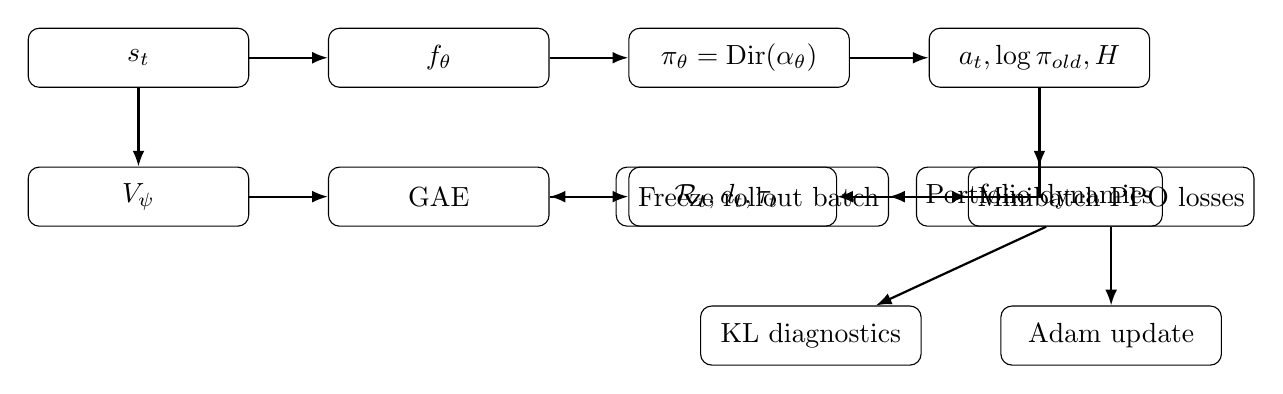
\begin{tikzpicture}[
  node distance=1.0cm,
  box/.style={draw, rounded corners, align=center, minimum width=2.8cm, minimum height=0.75cm},
  arrow/.style={-{Latex[length=2mm]}, thick}
]
\node[box] (s) {$s_t$};
\node[box, right=of s] (actor) {$f_\theta$};
\node[box, right=of actor] (dir) {$\pi_\theta=\mathrm{Dir}(\alpha_\theta)$};
\node[box, right=of dir] (a) {$a_t,\log\pi_{old},H$};
\node[box, below=of a] (env) {Portfolio dynamics};
\node[box, left=of env] (r) {$\mathcal{R}_t,d_t,\tau_t$};
\node[box, below=of s] (critic) {$V_\psi$};
\node[box, right=of critic] (gae) {GAE};
\node[box, right=of gae] (freeze) {Freeze rollout batch};
\node[box, right=of freeze] (loss) {Minibatch PPO losses};
\node[box, below=of loss] (update) {Adam update};
\node[box, left=of update] (kl) {KL diagnostics};
\draw[arrow] (s) -- (actor);
\draw[arrow] (actor) -- (dir);
\draw[arrow] (dir) -- (a);
\draw[arrow] (a) -- (env);
\draw[arrow] (env) -- (r);
\draw[arrow] (s) -- (critic);
\draw[arrow] (critic) -- (gae);
\draw[arrow] (r) -- (gae);
\draw[arrow] (gae) -- (freeze);
\draw[arrow] (a) |- (freeze);
\draw[arrow] (freeze) -- (loss);
\draw[arrow] (loss) -- (update);
\draw[arrow] (loss) -- (kl);
\end{tikzpicture}
}
\caption{Regime-aware PPO optimization on the portfolio simplex. Rollout
quantities are frozen before minibatch PPO epochs; Adam state persists across
updates and approximate KL controls early stopping.}
\end{figure}

\subsection{Training Algorithm}

Algorithmically, one train split is optimized as follows:
\begin{enumerate}[leftmargin=*]
  \item Initialize actor parameters $\theta$, critic parameters $\psi$, and
  Adam optimizer state.
  \item Roll out the current policy through the functional trading environment
  over the train split, storing $(s_t,a_t,\log\pi_{\theta}(a_t\mid s_t),
  \mathcal{R}_t,V_\psi(s_t),d_t,\tau_t)$.
  \item Compute GAE using the stored rewards, terminal masks, and stored critic
  values. Form returns $G_t=A_t+V_\psi(s_t)$ and normalize advantages once
  over the full rollout.
  \item Freeze the rollout batch, including old log probabilities and old
  values.
  \item For each PPO epoch, deterministically shuffle indices
  $\{1,\ldots,T\}$ and split them into minibatches.
  \item For each minibatch, minimize the clipped actor-critic loss, apply
  global gradient norm clipping, update parameters with Adam, and record
  diagnostics.
  \item Stop early if approximate KL exceeds the configured target.
  \item Return a checkpoint containing actor parameters, critic parameters,
  optimizer state, train-window metadata, and configuration.
\end{enumerate}

The implementation currently performs this procedure for one collected rollout
per train split. This is intentionally simple: it makes the train/evaluate
boundary easy to audit and keeps the unit tests focused on the accounting and
PPO update invariants. A larger empirical system could repeat the rollout and
update cycle multiple times within the train split, provided every rollout
still uses only train-period data.

\section{Theoretical Properties}

\begin{assumption}[Causal observability]
At decision time $t$, the feature window, benchmark history, portfolio context,
and HMM filtering posterior are measurable with respect to the market filtration
$\mathcal{F}_t$.
\end{assumption}

\begin{proposition}[No smoothing leakage]
If $p_t(k)$ is computed by the forward HMM recursion using observations
$\phi_{1:t}$ only, then $p_t$ is $\mathcal{F}_t$-measurable and does not depend
on future observations $\phi_{t+1:T}$.
\end{proposition}

\begin{proof}
The forward recursion initializes from fixed model parameters and updates
$\alpha_t$ using $\alpha_{t-1}$ and the emission likelihood of $\phi_t$. By
induction, $\alpha_{t-1}$ is a function only of $\phi_{1:t-1}$; therefore
$\alpha_t$, and its normalized probability vector $p_t$, is a function only of
$\phi_{1:t}$. No term in the recursion references $\phi_{t+1:T}$.
\end{proof}

\begin{proposition}[Causal policy action]
Assume the feature windows, fitted preprocessing parameters, encoder
parameters, HMM parameters, and portfolio context available at time $t$ are
$\mathcal{F}_t$-measurable. If the actor parameters $\theta$ are fixed before
the decision and the sampling key is independent of future market returns, then
the sampled action $a_t$ is generated without using future market information.
\end{proposition}

\begin{proof}
By assumption, the inputs to $g_\eta$ are $\mathcal{F}_t$-measurable, so
$\phi_t=g_\eta(\cdot)$ is $\mathcal{F}_t$-measurable. By the filtering
proposition, $p_t$ is also $\mathcal{F}_t$-measurable. The portfolio context is
carried from prior environment states and is therefore known at the decision
time. Hence $s_t$ is $\mathcal{F}_t$-measurable. The actor maps $s_t$ to
Dirichlet parameters deterministically, and the only remaining randomness is
the policy sampling key, which is independent of future returns. Therefore
$a_t$ cannot be a function of $\phi_{t+1:T}$ or future realized returns.
\end{proof}

\begin{proposition}[Simplex feasibility]
For $\alpha_i>0$ for all $i$, a Dirichlet policy samples actions in the
long-only simplex almost surely.
\end{proposition}

\begin{proof}
The support of the Dirichlet distribution with strictly positive concentration
parameters is the open probability simplex. Since
$\alpha_i=c\mu_i+\alpha_{\min}$ and $\alpha_{\min}>0$, all concentrations are
strictly positive. Thus sampled weights satisfy $a_i>0$ and $\sum_i a_i=1$
almost surely.
\end{proof}

\begin{proposition}[Frozen old log probabilities are required for PPO ratios]
Let $a_t$ be sampled from $\pi_{\theta_{\mathrm{old}}}(\cdot\mid s_t)$. The
importance ratio $r_t(\theta)$ is a valid likelihood ratio between the new
policy and the data-generating policy only if the denominator remains
$\pi_{\theta_{\mathrm{old}}}(a_t\mid s_t)$ throughout the PPO epochs.
\end{proposition}

\begin{proof}
The change-of-measure identity for any integrable function $h$ is
\[
\E_{a\sim\pi_{\theta_{\mathrm{old}}}}
\left[
\frac{\pi_\theta(a\mid s_t)}
{\pi_{\theta_{\mathrm{old}}}(a\mid s_t)}
h(a)
\right]
=
\E_{a\sim\pi_\theta}[h(a)].
\]
This identity uses the distribution that actually generated the sampled action
in the denominator. If the denominator is recomputed after updating parameters,
it no longer represents the sampling distribution of the fixed data. The ratio
then ceases to be an importance weight, and PPO's clipped objective loses its
intended interpretation as a conservative update from the rollout policy.
\end{proof}

\begin{proposition}[Bounded one-step transaction-cost penalty]
For $w,w'\in\simplex$ and transaction cost rate $\rho\ge0$, the transaction
cost $c=\rho\sum_i|w'_i-w_i|$ satisfies $0\le c\le 2\rho$.
\end{proposition}

\begin{proof}
The $\ell_1$ distance between any two probability vectors is at most $2$ and at
least $0$. Multiplying by $\rho$ yields the bound.
\end{proof}

These propositions are deliberately modest. They do not claim convergence of
PPO in non-stationary markets. Instead, they establish feasibility and causal
validity of the state-action construction, which are prerequisites for credible
empirical study.

\section{Reference Implementation}

The reference implementation instantiates the above framework in small modules:
\begin{itemize}[leftmargin=*]
  \item Causal lookback construction:
  \pathref{src/finrl/models/windows.py}.
  \item Market encoder:
  \pathref{src/finrl/models/encoder.py}.
  \item Filtering HMM:
  \pathref{src/finrl/regimes/filtering.py}.
  \item PPO policy and value networks:
  \pathref{src/finrl/ppo/policy.py} and
  \pathref{src/finrl/ppo/value.py}.
  \item Dirichlet policy distribution:
  \pathref{src/finrl/ppo/distributions.py}.
  \item GAE and PPO losses:
  \pathref{src/finrl/ppo/gae.py} and
  \pathref{src/finrl/ppo/losses.py}.
  \item PPO rollout collection, frozen update batches, minibatch optimization,
  optimizer state, KL stopping, and diagnostics:
  \pathref{src/finrl/ppo/trainer.py}.
  \item Functional trading environment:
  \pathref{src/finrl/env/trading_env.py} and
  \pathref{src/finrl/env/accounting.py}.
  \item Strict walk-forward orchestration:
  \pathref{src/finrl/experiments/run_walk_forward.py}.
\end{itemize}

The module boundaries mirror the mathematical decomposition. Data and feature
code produce causal observations; encoder code maps windows to $\phi_t$; regime
code maps embeddings to filtering posteriors; environment code implements the
accounting transition; and PPO code consumes the resulting state, action,
reward, and value tensors. This separation is intentional. It makes it possible
to test financial invariants, such as turnover and cash accounting, separately
from policy-gradient machinery.

The important tensor shapes are summarized in Table~\ref{tab:shapes}.

\begin{table}[ht]
\centering
\begin{tabular}{lll}
\toprule
Quantity & Symbol / Name & Shape \\
\midrule
Asset window & $X^{asset}$ & $(T,L,A,F_a)$ \\
Macro window & $X^{macro}$ & $(T,L,F_m)$ \\
Spectral row & $X^{spectral}$ & $(T,20)$ \\
Market embedding & $\phi$ & $(T,32)$ \\
Regime posterior & $p$ & $(T,K)$ \\
Asset returns & $R$ & $(T,N)$ \\
PPO state & $s$ & $(T,32+K+N+2)$ \\
Action weights & $a$ & $(T,N)$ \\
Log probabilities & $\log\pi$ & $(T,)$ \\
Rewards & $\mathcal{R}$ & $(T,)$ \\
Values & $V$ & $(T,)$ \\
Advantages, returns & $A,G$ & $(T,)$ \\
Minibatch indices & $\mathcal{I}_b$ & $(B,)$ \\
Diagnostics & policy/value loss, KL, entropy, turnover & scalar per update \\
\bottomrule
\end{tabular}
\caption{Principal tensor shapes. $T$ is split length, $L$ is lookback, $A$ is
the number of encoder assets, $F_a$ and $F_m$ are feature dimensions, $K$ is the
number of regimes, and $N$ is the tradable asset count.}
\label{tab:shapes}
\end{table}

\section{Experimental Protocol}

A credible empirical evaluation should use strict walk-forward testing. For each
split, preprocessing artifacts, HMM parameters, and policy parameters are fit on
the train period only. The resulting checkpoint is frozen and evaluated on the
subsequent test period. Metrics should include cumulative return, annualized
return, volatility, maximum drawdown, mean turnover, total transaction cost, and
benchmark-relative alpha.

The reference implementation currently supports this protocol structurally. The
encoder objective, however, is intentionally unspecified; therefore experiments
using the current code should report that encoder weights are randomly
initialized unless a training objective is added.

During each train split, PPO first collects an on-policy rollout through the
same functional trading environment used for evaluation. It then constructs a
frozen update batch containing states, sampled actions, old action log
probabilities, rewards, old critic values, GAE advantages, and value targets.
The advantages are normalized once at rollout scope. PPO update epochs shuffle
the frozen rollout indices with deterministic JAX PRNG handling and apply
minibatch updates. The returned training result exposes diagnostics for policy
loss, value loss, entropy, total loss, approximate KL, clip fraction, explained
variance, mean reward, mean turnover, maximum drawdown, completed epochs, and
completed optimizer updates.

Each diagnostic has a distinct role:
\begin{itemize}[leftmargin=*]
  \item Policy loss measures the clipped surrogate objective and should be
  interpreted relative to advantage scaling, not as a financial return.
  \item Value loss and explained variance measure critic fit. A weak critic can
  increase policy-gradient variance even if the actor loss looks finite.
  \item Entropy measures action-distribution spread on the simplex. It helps
  distinguish deliberate concentration from premature collapse.
  \item Approximate KL and clip fraction measure how far PPO updates move from
  the rollout policy. Large values indicate that the optimization phase may be
  overusing stale rollout data.
  \item Mean reward, mean turnover, and maximum drawdown connect optimizer
  behavior back to financial accounting.
\end{itemize}

The unit tests therefore cover both sides of the system. Accounting tests verify
portfolio value evolution, turnover, transaction cost, drawdown, cash
accounting, and weekly rebalance behavior. PPO tests verify action simplex
validity, stable advantage normalization, frozen old log probabilities, KL
early stopping, clipped value loss, persistent optimizer state, and a small
deterministic two-asset convergence fixture. The fixture is intentionally
simple: asset $0$ has a constant positive return and asset $1$ has lower
return, so a working policy update should increase the mean allocation to asset
$0$ without producing NaNs.

\section{Limitations and Future Work}

The current PPO trainer now includes the principal stabilization mechanisms
expected of a compact PPO implementation: persistent Adam state, global gradient
norm clipping, rollout-level advantage normalization, frozen old log
probabilities and value targets across epochs, shuffled minibatches, value
clipping, approximate KL monitoring, and early stopping. It remains intentionally
small and auditable. Important future work includes:
\begin{enumerate}[leftmargin=*]
  \item repeated rollout collection over multiple policy iterations within a
  train split, rather than a single rollout followed by PPO epochs;
  \item explicit cash semantics in the environment when cash is not already
  represented as a return column;
  \item a documented encoder training objective;
  \item richer train/test reporting that persists PPO diagnostics alongside
  portfolio metrics;
  \item ablations for regimes, transaction costs, drawdown penalties, and
  Dirichlet concentration.
\end{enumerate}

There is also a subtle accounting convention: turnover is implemented as the
full $\ell_1$ distance between old and new weights. Some portfolio literature
defines one-way turnover as half this value. Empirical claims should therefore
state the convention explicitly.

\section{Conclusion}

We presented a theoretical formulation of regime-aware PPO for long-only
portfolio control and connected it to an auditable JAX reference implementation.
The framework combines causal representation learning, filtering-only regime
inference, simplex-valued stochastic policies, and walk-forward evaluation. The
result is not yet a fully mature empirical trading system, but it is a coherent
research substrate: the state, action, reward, policy density, advantage
estimator, and PPO objective are explicit, inspectable, and compatible with
deterministic backtesting. This transparency is a necessary foundation for
future empirical claims about reinforcement learning in financial markets.

\end{document}
